\chapter{Results} % Main appendix title
\label{Appendix-results} % For referencing this appendix elsewhere, use 

%%%%%%%%%%%%%%%%%%%%%%%%%%%%%%%%%%%%%%%%%%%%%%%%%%%%%%%%%%%%%%%%%%%%%%%%%%%%%
% RUN XX - TEMPLATE - experiment log template
%%%%%%%%%%%%%%%%%%%%%%%%%%%%%%%%%%%%%%%%%%%%%%%%%%%%%%%%%%%%%%%%%%%%%%%%%%%%%
%\subsection{Run XX -  }
%\label{app_res:XX}
%\begin{verbatim}
%Commit:
%Model: 
%Outputs: 
%Dataset: 
%Command:
%Environment: 
%Comment: 
%\end{verbatim}

%%%%%%%%%%%%%%%%%%%%%%%%%%%%%%%%%%%%%%%%%%%%%%%%%%%%%%%%%%%%%%%%%%%%%%%%%%%%%
% RUN 01 
%%%%%%%%%%%%%%%%%%%%%%%%%%%%%%%%%%%%%%%%%%%%%%%%%%%%%%%%%%%%%%%%%%%%%%%%%%%%%

\subsection{Run 01 - RealSense Viewer}
\label{app_res:01}

Trying RealSense Viewer with the D415 camera.

Started RealSense Viewer (v2.45.0): 
\begin{verbatim}
$ realsense-viewer    
\end{verbatim}
Updated camera firmware to version 5.12.13.50 from 05.12.11.00.  

Screen capture uploaded to \Url{https://youtu.be/eltQ_hvpcFs}
Figure \ref{fig:RealSenseViewer2} shows the RGB Camera capture on the left and the Stereo Module Depth capture on the right, of the RealSense Viewer desktop application, which also allows saving captures to point cloud .ply files.

\begin{figure}[h!]
\centering
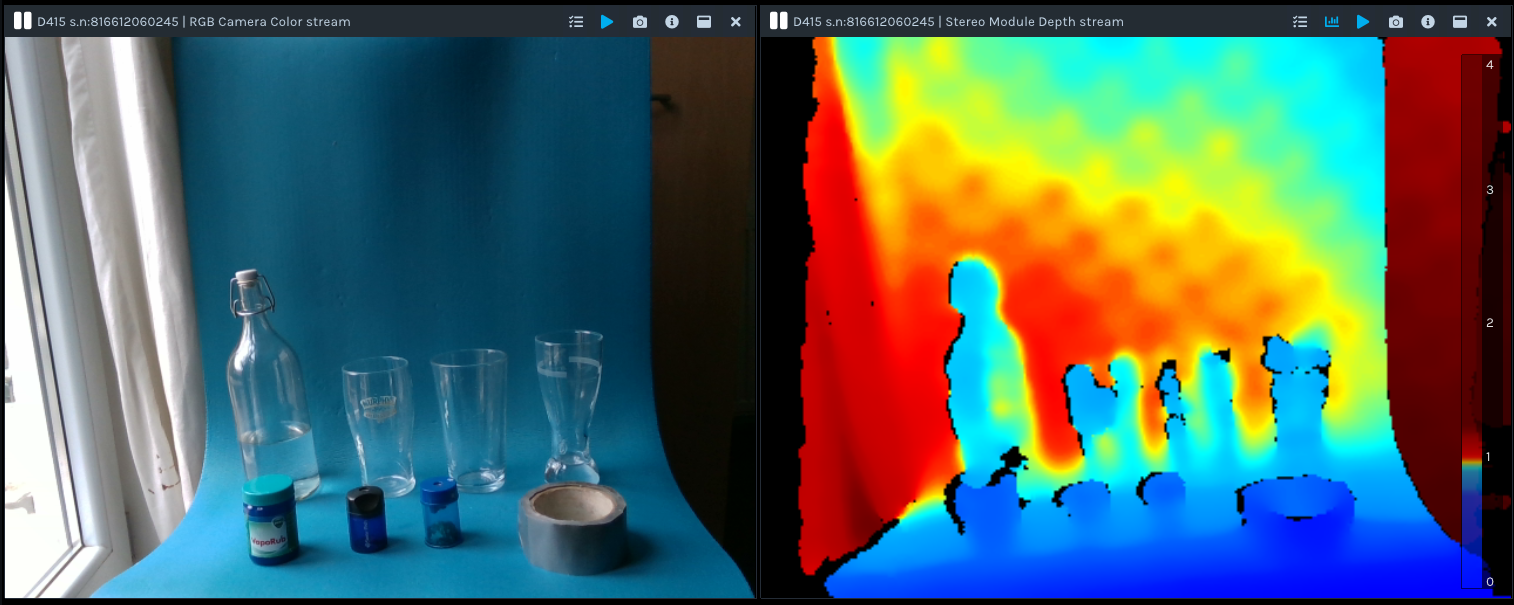
\includegraphics[width=\textwidth]{Figures/RealSenseViewer2.png}
\caption{RealSense Viewer desktop application}
\label{fig:RealSenseViewer2}
\end{figure}
Using RealSense Viewer, we output 3 files: output\_meshing\_no\_normals.ply, output\_meshing\_normals.ply and output\_no\_meshing\_no\_normals.ply.
% Kazam 
% Windows key + CTRL + R = Start recording.
% Windows key + CTRL + P = Pause recording, press again to resume.
% Windows key + CTRL + F = Finish recording.
% Windows key + CTRL + Q = Quit recording.

%%%%%%%%%%%%%%%%%%%%%%%%%%%%%%%%%%%%%%%%%%%%%%%%%%%%%%%%%%%%%%%%%%%%%%%%%%%%%
% RUN 02 
%%%%%%%%%%%%%%%%%%%%%%%%%%%%%%%%%%%%%%%%%%%%%%%%%%%%%%%%%%%%%%%%%%%%%%%%%%%%%

\subsection{Run 02 - Viewing Realsense Viewer point cloud output using Open3D}
\label{app_res:02}
\begin{verbatim}
File: ~/git/cleargrasp/live_demo/viz/display-point-cloud.py
Commit: fb79cdc
Point cloud file: ~/git/cleargrasp/live_demo/viz/data/output_meshing_normals.ply
\end{verbatim}
 We then visualise with Open3D:
\begin{verbatim}
# ~/git/cleargrasp/live_demo/viz
# from open3d import *    
import open3d as o3d

def main():
    # Read the point cloud
    cloud = o3d.io.read_point_cloud("output_meshing_normals.ply") 
    # Visualize the point cloud   
    o3d.visualization.draw_geometries([cloud])   

if __name__ == "__main__":
    main()
\end{verbatim}

The output provides a mean of performing qualitative analysis on cleargrasp depth completion.
\begin{figure}[h!]
\centering
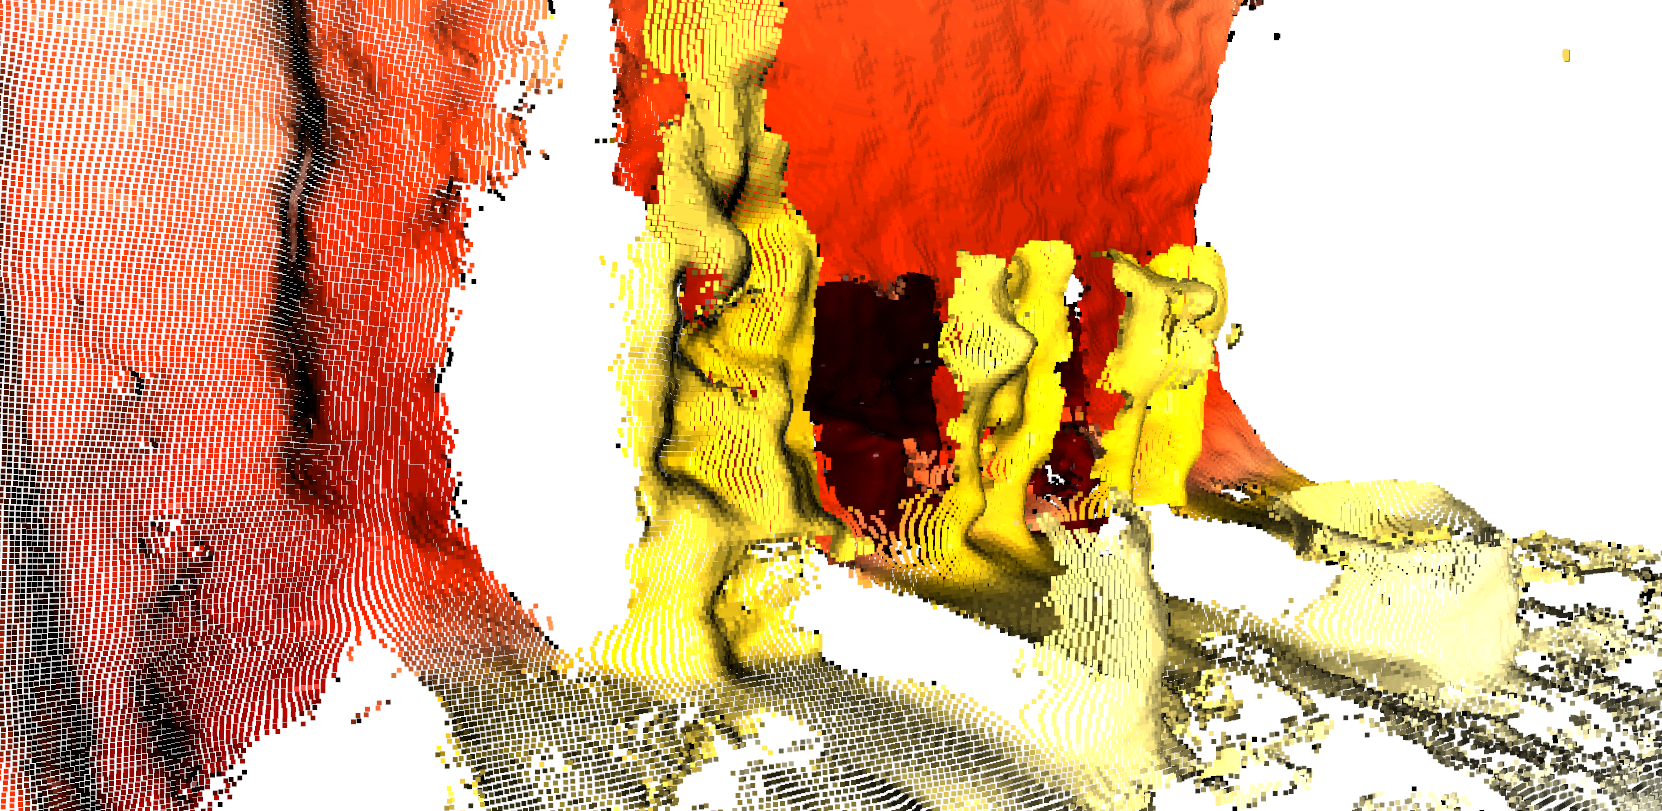
\includegraphics[width=\textwidth]{Figures/OpenCV-point-cloud-import-2.png}
\caption{RealSense Viewer D415 point cloud output rendered with OpenCV}
\label{fig:realsenseOutputForReport1}
\end{figure}
The image shows clear surfaces (bottle and glasses) are deformed, while the tub and tape roll are not.
%%%%%%%%%%%%%%%%%%%%%%%%%%%%%%%%%%%%%%%%%%%%%%%%%%%%%%%%%%%%%%%%%%%%%%%%%%%%%
% RUN 03 
%%%%%%%%%%%%%%%%%%%%%%%%%%%%%%%%%%%%%%%%%%%%%%%%%%%%%%%%%%%%%%%%%%%%%%%%%%%%%

\subsection{Run 03 - Using Zivid Studio}
\label{app_res:03}
Zivid Studio is a desktop application that provides a point and click interface to control Zivid camera acquisitions, as well as save outputs. A screen capture can be seen at  Url{https://youtu.be/YYi-erfRAFw}.
Figure \ref{fig:ZividStudioDetail} shows a detail of the 3D Point Cloud capture in Zivid Studio.
\begin{figure}[h!]
\centering
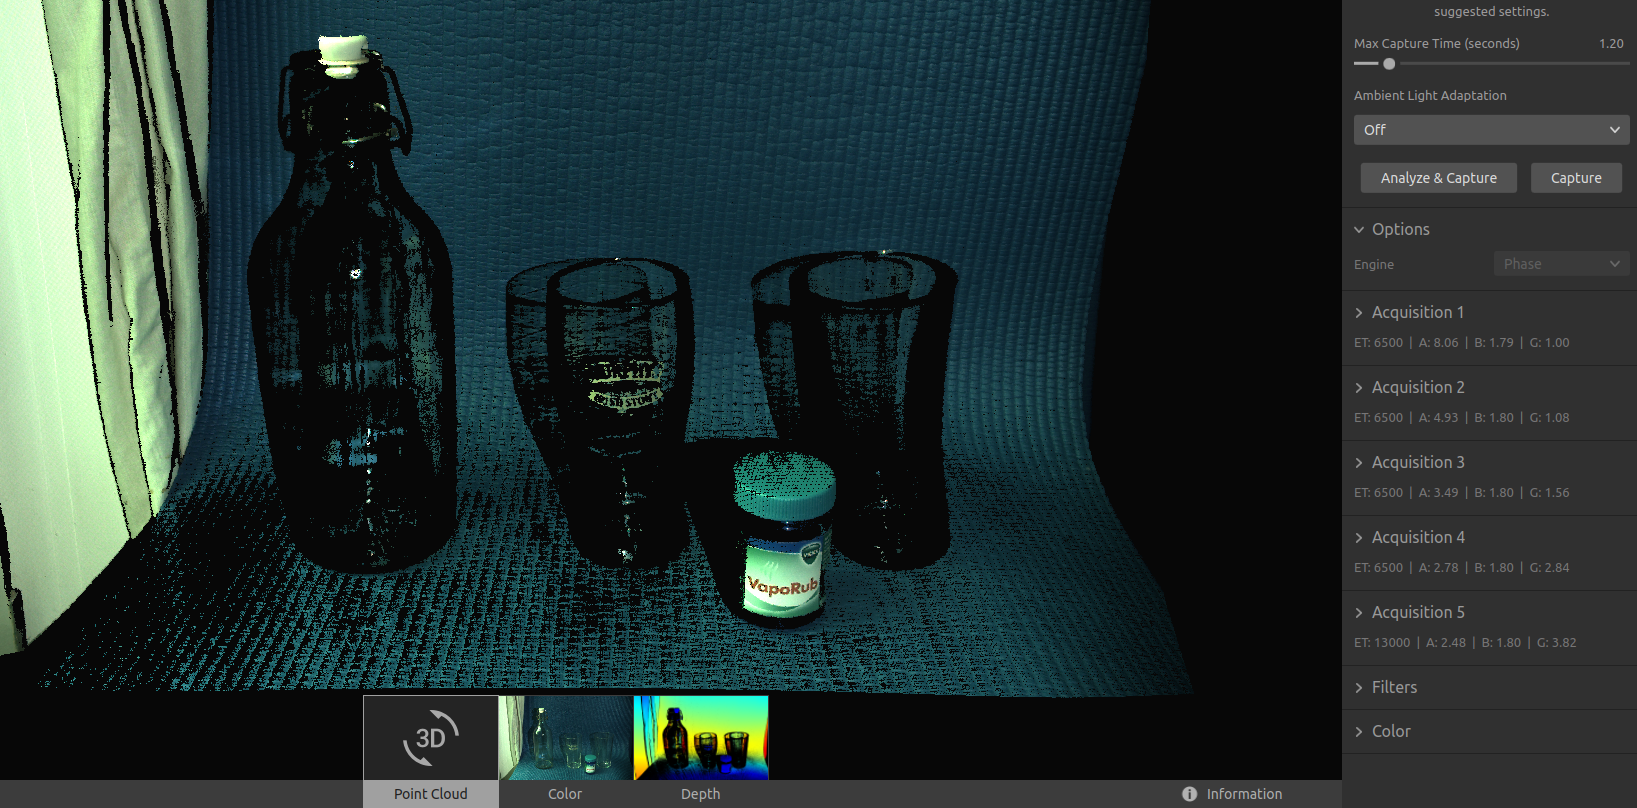
\includegraphics[width=\textwidth]{Figures/ZividStudioDetail.png}
\caption{Zivid Studio detail}
\label{fig:ZividStudioDetail}
\end{figure}
A point cloud output was saved to data/zivid\_studio\_capture.ply.

%%%%%%%%%%%%%%%%%%%%%%%%%%%%%%%%%%%%%%%%%%%%%%%%%%%%%%%%%%%%%%%%%%%%%%%%%%%%%
% RUN 04 
%%%%%%%%%%%%%%%%%%%%%%%%%%%%%%%%%%%%%%%%%%%%%%%%%%%%%%%%%%%%%%%%%%%%%%%%%%%%%

\subsection{Run 04 - Viewing Zivid Studio point cloud output using Open3D}
\label{app_res:04}
\begin{verbatim}
Script file: ~/git/cleargrasp/live_demo/viz/display-point-cloud.py
Commit: 6c7076f
Point cloud file: ~/git/cleargrasp/live_demo/viz/data/zivid_studio_capture.ply
We also ran another script:
Commit: bc314bd
With an added point cloud transform that corrects the viewer orientation.
\end{verbatim}
Figure \ref{fig:ZividOpen3DPointCloud} shows the Zivid Point cloud generated in run \ref{app_res:03} rendered with Open3D, showing that transparent objects were not rendered correctly.

\begin{figure}[h!]
\centering
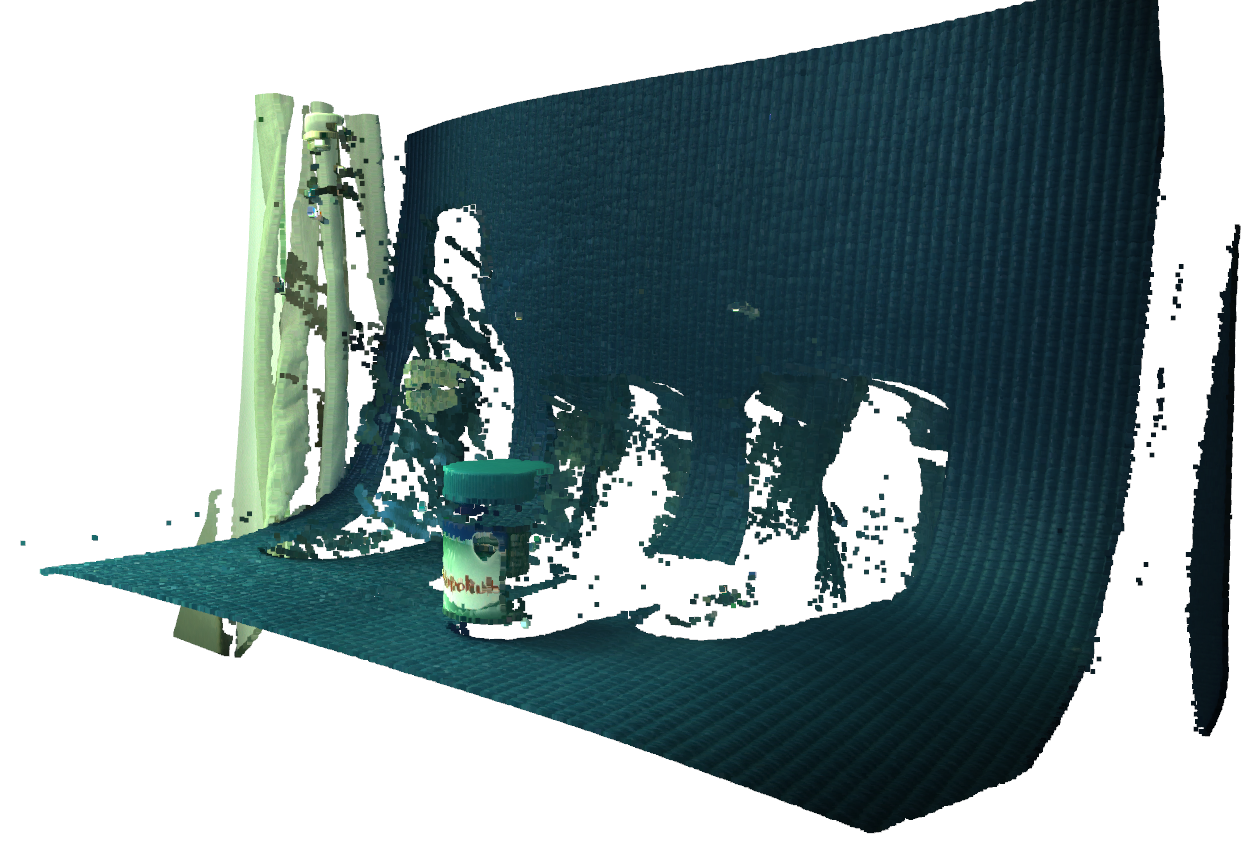
\includegraphics[width=\textwidth]{Figures/ZividOpen3DPointCloud.png}
\caption{Zivid Point Cloud rendered with Open3D}
\label{fig:ZividOpen3DPointCloud}
\end{figure}


%%%%%%%%%%%%%%%%%%%%%%%%%%%%%%%%%%%%%%%%%%%%%%%%%%%%%%%%%%%%%%%%%%%%%%%%%%%%%
% RUN 05 - D415 live demo
%%%%%%%%%%%%%%%%%%%%%%%%%%%%%%%%%%%%%%%%%%%%%%%%%%%%%%%%%%%%%%%%%%%%%%%%%%%%%

\subsection{Run 05 - D415 Live Demo}
We ran the live Demo, and saved image and numpy array files for RGB and depth.
\label{app_res:05}
\begin{verbatim}
Commit: 61dbc03
Command:
$ python live_demo.py -c config/config.yaml
Outputs:
D415-rbg-input.png
d415_color_img.npy
d415_input_depth.npy
\end{verbatim}

\begin{verbatim}
(...)
from realsense import camera    
(...)
rcamera = camera.Camera()
(...)
# Get Frame. Expected format: ColorImg -> (H, W, 3) uint8, DepthImg -> (H, W) float64
color_img, input_depth = rcamera.get_data()
(..)
# save images and numpy arrays
im = Image.fromarray(color_img)
im.save("D415-rbg-input.png")
# cannot save depth as png
# im = Image.fromarray(input_depth)
# im.save("D415-depth-input.png")

input_depth = input_depth.astype(np.float32)
with open('d415_color_img.npy', 'wb') as f:
    np.save(f, color_img)
with open('d415_input_depth.npy', 'wb') as f:
    np.save(f, input_depth)

\end{verbatim}

Figure \ref{fig:ClearGraspLiveDemoForReport} shows the input on top left, then predicted surface normals and boundaries. On the bottom row, from the left is the transparent object mask, output depth mapped and filtered output depth mapped, followed by a blank image to make up the rows and columns.

\begin{figure}[h!]
\centering
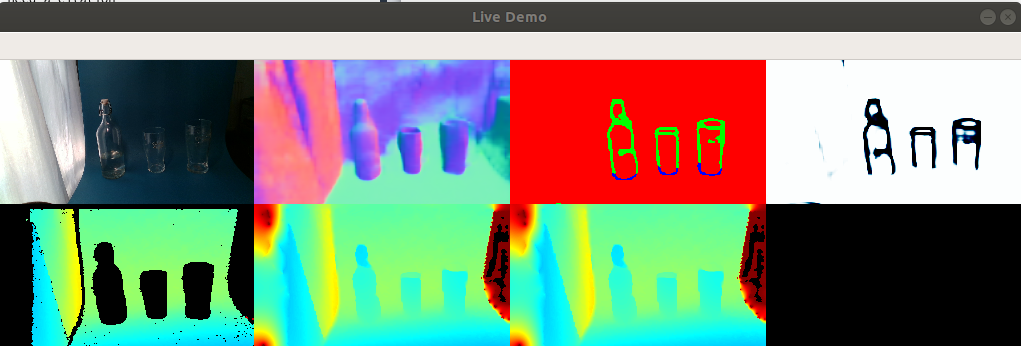
\includegraphics[width=\textwidth]{Figures/ClearGraspLiveDemoForReport.png}
\caption{ClearGrasp live demo with the D415 camera}
\label{fig:ClearGraspLiveDemoForReport}
\end{figure}

%%%%%%%%%%%%%%%%%%%%%%%%%%%%%%%%%%%%%%%%%%%%%%%%%%%%%%%%%%%%%%%%%%%%%%%%%%%%%
% RUN 06  - Zivid One+ live demo
%%%%%%%%%%%%%%%%%%%%%%%%%%%%%%%%%%%%%%%%%%%%%%%%%%%%%%%%%%%%%%%%%%%%%%%%%%%%%

\subsection{Run 06 - Zivid One+ Live Demo}
\label{app_res:06}

\begin{verbatim}
Commit: 741469e
Command:
$ python zivid_live_demo.py -c config/config.yaml
Running live demo of depth completion. Make sure Zivid One+ camera is connected.

Saving captured images to folder: "../data/captures/exp-002"

 Press "c" to capture and save image, press "q" to quit

Creating DRN model for normals and loading checkpoint
Creating DRN model for outlines and loading checkpoint
Creating DRN model for masks and loading checkpoint
(...)

Outputs:
zivid_color_img.npy
zivid_input_depth.npy
zivid-rbg-input.png

\end{verbatim}

% $ python zivid_live_demo.py -c config/config.yaml
% $ python zivid_live_demo.py -c config/config.yaml
% Running live demo of depth completion. Make sure Zivid One+ camera is connected.

% Saving captured images to folder: "../data/captures/exp-002"

% Press "c" to capture and save image, press "q" to quit

% Creating DRN model for normals and loading checkpoint
% Creating DRN model for outlines and loading checkpoint
% Creating DRN model for masks and loading checkpoint

Figure \ref{fig:ZividLiveDemo} shows the \ref{app_res:05} Zivid One+ live demo equivalent. With following distinctions, the D415 outputs are accessed using the camera function from the realsense module in live\_demo.py, while the Zivid script uses the zivid python library.



\begin{figure}[h!]
\centering
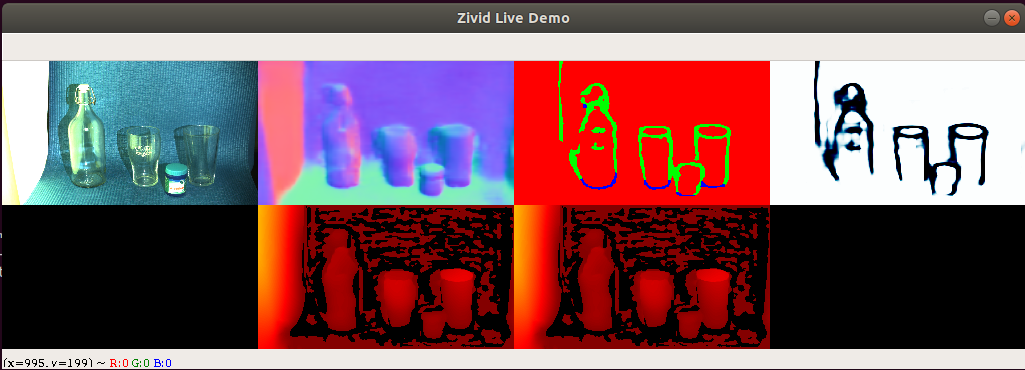
\includegraphics[width=\textwidth]{Figures/ZividLiveDemo.png}
\caption{ClearGrasp live demo with the Zivid One+ camera}
\label{fig:ZividLiveDemo}
\end{figure}

We notice that the no masks (bottom left) have been generated. The code to zivid\_live\_demon.py makes use of a separate script, to substitute the realsense camera function. The script zivid\_utils:
\begin{verbatim}
point_cloud = frame.point_cloud()
# get rgb data
rgba = point_cloud.copy_data("rgba")
rgb = rgba[:, :, 0:3]
zivid_rgb = cv2.resize(rgb, (1280, 720))
# get depth data
z = frame.point_cloud().copy_data("z")
zivid_input_depth = np.asarray(z)
zivid_input_depth = cv2.resize(zivid_input_depth, (1280, 720))
\end{verbatim}
From the point cloud acquisition, the RGB data is saved, and the A channel discarded. The depth data is also saved, both RGB and depth as numpy arrays and both resized to 1280 x 720 pixels, which is the size expected by the trained networks.

% visualise saved numpy arrays
%%%%%%%%%%%%%%%%%%%%%%%%%%%%%%%%%%%%%%%%%%%%%%%%%%%%%%%%%%%%%%%%%%%%%%%%%%%%%
% RUN 07 - Plotting D415 and Zivid One+ RGB and depth numpy arrays
%%%%%%%%%%%%%%%%%%%%%%%%%%%%%%%%%%%%%%%%%%%%%%%%%%%%%%%%%%%%%%%%%%%%%%%%%%%%%
\subsection{Run 07 - Plotting RGB and Depth from saved numpy arrays}
\label{app_res:07}
\begin{verbatim}
Commit: bf6f1dd
Command: VisualiseInputOutput.ipynb
\end{verbatim}
We ran a Jupyter Notebook to plot saved numpy arrays. In figure \ref{fig:D415-Zivid-RBG-Depth-From-Saved-Numpy-Arrays} on the top row are the D415 RBG and depth outputs, and on the bottom row, the Zivid One+ corresponding images. We note the RGB images are relatively similar, while the depth images are not.

\begin{figure}[h!]
\centering
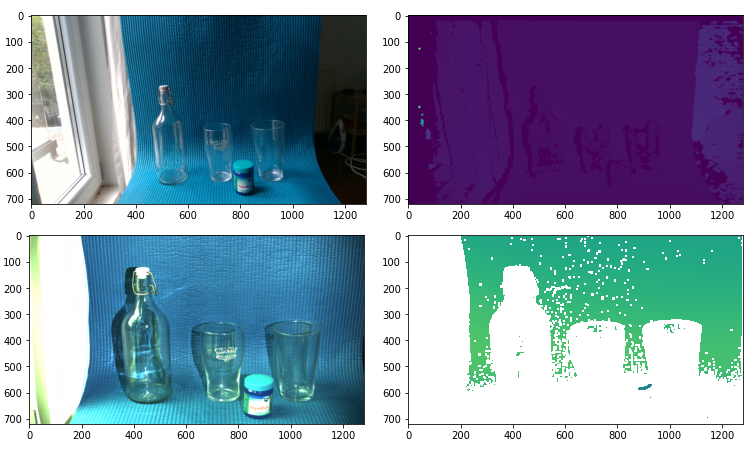
\includegraphics[width=\textwidth]{Figures/D415-Zivid-RBG-Depth-From-Saved-Numpy-Arrays.png}
\caption{D415 and Zivid One+ RGB and depth plots on top and bottom rows respectively}
\label{fig:D415-Zivid-RBG-Depth-From-Saved-Numpy-Arrays}
\end{figure}

We then studied the data and found that the zivid input depth in this case had approximately \%45 NAN (not a number) null values:
\begin{verbatim}
# D415
print(type(d415_input_depth)) # <class 'numpy.ndarray'>
print(d415_input_depth.shape) # (720, 1280)
print(type(d415_input_depth[0,0])) # <class 'numpy.float32'>
print(np.amin(d415_input_depth)) # 0.0
print(np.amax(d415_input_depth)) # 18.632

# First we need to clean up the zivid one data
# Zivid One+
print(type(zivid_input_depth)) # <class 'numpy.ndarray'>
print(zivid_input_depth.shape) # (720, 1280)
print(type(zivid_input_depth[0,0])) # <class 'numpy.float32'>
print(np.amin(zivid_input_depth)) # nan
print(np.amax(zivid_input_depth)) # nan
print(np.count_nonzero(np.isnan(zivid_input_depth))) # 412962, 720 * 1280 = 921600 ~ 45% nan    
\end{verbatim}
We removed the nan values:
\begin{verbatim}
# remove nans
zivid_input_depth = np.nan_to_num(zivid_input_depth)
print(np.amin(zivid_input_depth)) # 0.0
print(np.amax(zivid_input_depth)) # 1244.7163
\end{verbatim}
And noticed that the pixel values for the zivid capture were a log higher.
We then scaled to the values of the D415 depth:
\begin{verbatim}
# scale to 18.632
sf = 18.632 / 1244.7163
print("Scale factor: ", sf)
scaled_zivid_input_depth = zivid_input_depth * sf
print(np.amin(scaled_zivid_input_depth)) # 0.0
print(np.amax(scaled_zivid_input_depth)) # 18.632
plt.imshow(scaled_zivid_input_depth)    
\end{verbatim}
At this stage we observed that the resulting depth image as seen in figure \ref{fig:Scaled-Zivid-Depth} has a closer resemblance to the Zivid Studio depth capture (compare with Figure \ref{fig:ZividStudio}).

\begin{figure}[h!]
\centering
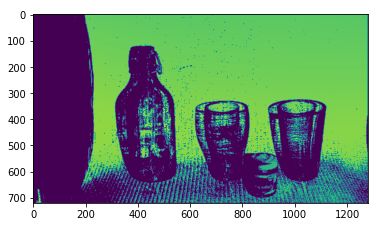
\includegraphics[width=\textwidth]{Figures/Scaled-Zivid-Depth.png}
\caption{Zivid One+ depth output scaled to D415 values}
\label{fig:Scaled-Zivid-Depth}
\end{figure}

These adjustments are not sufficient for the ClearGrasp pipeline to create the masks (commit 16d6778). We then plotted histograms of the values in both depth images as seen in Figure \ref{fig:Depth-Histograms}. We see the D415 depth has a narrower range, perhaps providing a clue on the adjustments required to the Zivid One+ depth output. We could sample from the ranges above 10, scale to three effectively shifting the values to the left to emulate the spike at 3 for D415 depth. A

\begin{figure}[h!]
\centering
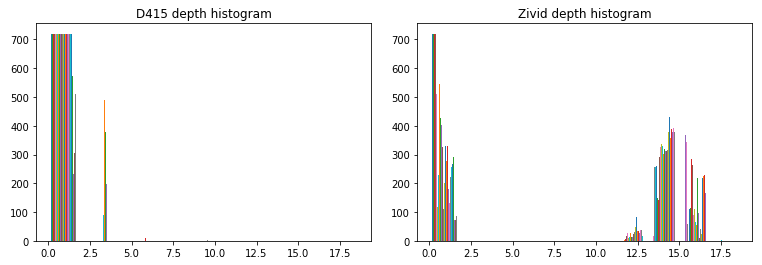
\includegraphics[width=\textwidth]{Figures/Depth-Histograms.png}
\caption{D415 and Zivid One+ depth histograms}
\label{fig:Depth-Histograms}
\end{figure}

%%%%%%%%%%%%%%%%%%%%%%%%%%%%%%%%%%%%%%%%%%%%%%%%%%%%%%%%%%%%%%%%%%%%%%%%%%%%%
% RUN 08 - D415 and Zivid One+ point cloud qualitative analysis
%%%%%%%%%%%%%%%%%%%%%%%%%%%%%%%%%%%%%%%%%%%%%%%%%%%%%%%%%%%%%%%%%%%%%%%%%%%%%

\subsection{Run 08 -  D415 and Zivid One+ point cloud qualitative analysis}
\label{app_res:08}
\begin{verbatim}
Commit: 9ed0861
Command: 
python display-point-cloud.py --file ZividStudioPointCloudCapture.ply --transform True
python display-point-cloud.py --file RealSenseViewerPointCloudCapture.ply
\end{verbatim}

We perform qualitative evaluation on D415 and Zivid One+ point cloud outputs (Figure \ref{fig:OpenCV-D415-Zivid-Point-Cloud}). Both show glass surfaces cannot be captured correctly. 

\begin{figure}[h!]
\centering
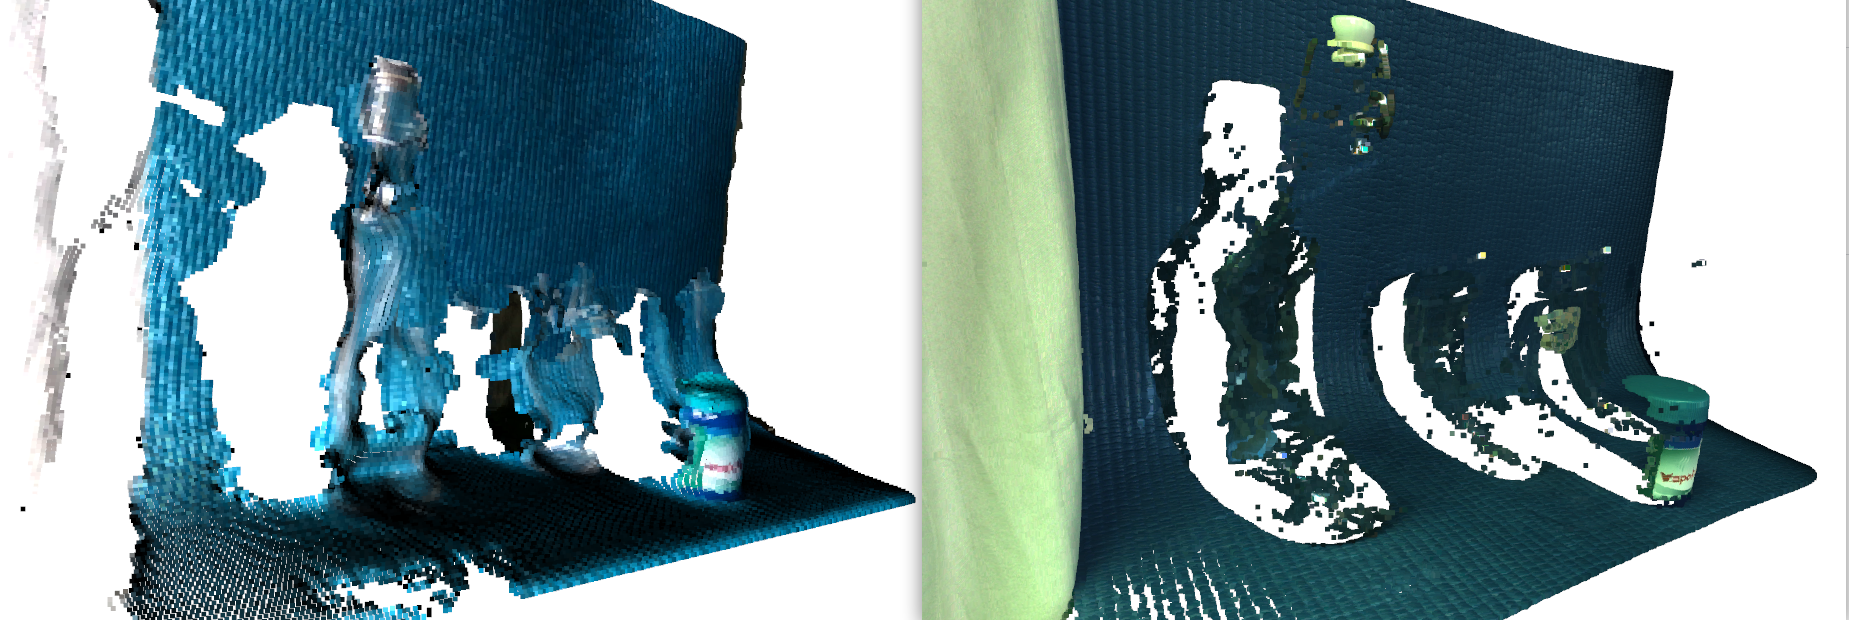
\includegraphics[width=\textwidth]{Figures/OpenCV-D415-Zivid-Point-Cloud.png}
\caption{D415 and Zivid One+ OpenCV point cloud renderings}
\label{fig:OpenCV-D415-Zivid-Point-Cloud}
\end{figure}

We notice that with the current settings, the D415 point cloud partially recreates the transparent geometries, specially the top back part of the glasses, while the bottom part follows approximately the (offset) geometry of the backdrop, which is curved between bottom and back surfaces. The bottle presents the same characteristics, except near the neck, where the curved profile is better defined in the point cloud. The Zivid One+ output (as per current settings) is approximately the same, except it fails to recreate the bottle geometry where it is curved near the neck, and also generates some noise behind the backdrop.

We should perhaps look at projection matrices used to generate the depth images. These are likely to be different in both environments (Intel, Zivid).

%%%%%%%%%%%%%%%%%%%%%%%%%%%%%%%%%%%%%%%%%%%%%%%%%%%%%%%%%%%%%%%%%%%%%%%%%%%%%
% RUN 09 - D415, Redwood and Zivid One+ point cloud data comparison
%%%%%%%%%%%%%%%%%%%%%%%%%%%%%%%%%%%%%%%%%%%%%%%%%%%%%%%%%%%%%%%%%%%%%%%%%%%%%
\subsection{Run 09 -  D415, Redwood and Zivid One+ point cloud data comparison}
\label{app_res:09}
We were able to generate a point cloud using script viz/create-point-cloud.py using RGB and depth files viz/color.png and viz/depth.png respectively. It turns out this have shape (1200, 1920, 4) and (1200, 1920, 3) respectively. We were not able to generate a point cloud using Redwood dataset files viz/001\_color.png and viz/001\_depth.png, with shapes (240, 320, 3) and (240, 320) respectively.

The saved numpy arrays for D415 and Zivid One+, using script live\_demo.py and zivid\_live\_demo.py have the same shape as Redwood data, i.e. (H, W, 3) for RGB and (H, W) for depth.

We are none the wiser in terms of generating a point cloud from these two files. Recapping, the reason we want to do this is to perform qualitative analysis on the completed depth, by generating a point cloud of the RGB and acquired depth and comparing it to a point cloud of the RGB and predicted depth.
\begin{verbatim}
Commit: d83278b
Command: 
Ran live\_demo/D415RedwoodZividDataComparison.ipynb notebook.
\end{verbatim}

%%%%%%%%%%%%%%%%%%%%%%%%%%%%%%%%%%%%%%%%%%%%%%%%%%%%%%%%%%%%%%%%%%%%%%%%%%%%%
% RUN 10 - Generating Point Cloud from D415 RGB and Depth outputs
%%%%%%%%%%%%%%%%%%%%%%%%%%%%%%%%%%%%%%%%%%%%%%%%%%%%%%%%%%%%%%%%%%%%%%%%%%%%%
\subsection{Run 10 -  Generating Point Cloud from D415 RGB and Depth outputs}
\label{app_res:10}
\begin{verbatim}
Commit: 400d0af
Command: 
python create-point-cloud.py
\end{verbatim}
We should now be able to perform qualitative analysis but comparing point clouds of depth camera output with predicted depth.
TODO. Add screen captures




% TODO write up links
% The Perspective and Orthographic Projection Matrix
% https://www.scratchapixel.com/lessons/3d-basic-rendering/perspective-and-orthographic-projection-matrix
% Projection in Intel RealSense SDK 2.0
% https://dev.intelrealsense.com/docs/projection-in-intel-realsense-sdk-20
% depth map from point cloud https://stackoverflow.com/questions/56288806/using-rgb-images-and-pointcloud-how-to-generate-depth-map-from-the-pointclouds
% From depth map to point cloud
% https://medium.com/yodayoda/from-depth-map-to-point-cloud-7473721d3f
% camera calibration
% https://medium.com/analytics-vidhya/camera-calibration-theory-and-implementation-b253dad449fb
% zivid point cloud .py
% https://github.com/zivid/zivid-python/blob/master/modules/zivid/point_cloud.py
% cleargrasp dataset
% https://github.com/Shreeyak/cleargrasp/tree/aspect_ratio_change/data/sample_dataset/real-val/d435
% deep completion
% https://github.com/yindaz/DeepCompletionRelease
% inte



%%%%%%%%%%%%%%%%%%%%%%%%%%%%%%%%%%%%%%%%%%%%%%%%%%%%%%%%%%%%%%%%%%%%%%%%%%%%%
% RUN XX - RGB and depth from point cloud outputs 
% Then compare with output generated by zivid_utils.py
%%%%%%%%%%%%%%%%%%%%%%%%%%%%%%%%%%%%%%%%%%%%%%%%%%%%%%%%%%%%%%%%%%%%%%%%%%%%%

%%%%%%%%%%%%%%%%%%%%%%%%%%%%%%%%%%%%%%%%%%%%%%%%%%%%%%%%%%%%%%%%%%%%%%%%%%%%%
% RUN 07 - D415 point cloud from depth and RGB
%%%%%%%%%%%%%%%%%%%%%%%%%%%%%%%%%%%%%%%%%%%%%%%%%%%%%%%%%%%%%%%%%%%%%%%%%%%%%
%\subsection{Run 06 - Zivid One+ Live Demo}
%\label{app_res:06}
%%%%%%%%%%%%%%%%%%%%%%%%%%%%%%%%%%%%%%%%%%%%%%%%%%%%%%%%%%%%%%%%%%%%%%%%%%%%%
% RUN 08 - Zivid One+ point cloud from depth and RGB
%%%%%%%%%%%%%%%%%%%%%%%%%%%%%%%%%%%%%%%%%%%%%%%%%%%%%%%%%%%%%%%%%%%%%%%%%%%%%
%\subsection{Run 06 - Zivid One+ Live Demo}
%\label{app_res:06}

%%%%%%%%%%%%%%%%%%%%%%%%%%%%%%%%%%%%%%%%%%%%%%%%%%%%%%%%%%%%%%%%%%%%%%%%%%%%%
% RUN 09 - Zivid One+ point cloud from predicteddepth and RGB
%%%%%%%%%%%%%%%%%%%%%%%%%%%%%%%%%%%%%%%%%%%%%%%%%%%%%%%%%%%%%%%%%%%%%%%%%%%%%

%%%%%%%%%%%%%%%%%%%%%%%%%%%%%%%%%%%%%%%%%%%%%%%%%%%%%%%%%%%%%%%%%%%%%%%%%%%%%
% RUN 10 - Zivid One+ point cloud from predicteddepth and RGB
%%%%%%%%%%%%%%%%%%%%%%%%%%%%%%%%%%%%%%%%%%%%%%%%%%%%%%%%%%%%%%%%%%%%%%%%%%%%%